\item \subquestionpointswritten{1}
For Dataset 1, compare the validation set plots obtained in part (b) and part (e)
from logistic regression and GDA respectively, and briefly comment on your observation in a couple of lines.\\[50pt]

\begin{figure}[H]
    \centering
    \begin{subfigure}{.5\textwidth}
      \centering
      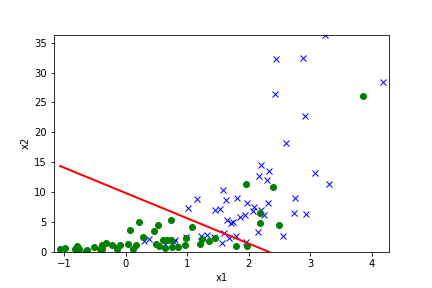
\includegraphics[width=0.95\linewidth]{./linearclass/src/lr_image1.png}
      \caption{Logistic Regression}
    \end{subfigure}%
    \begin{subfigure}{.5\textwidth}
      \centering
      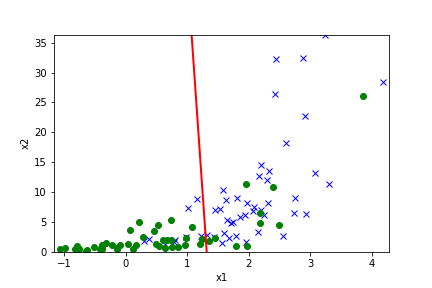
\includegraphics[width=0.95\linewidth]{./linearclass/src/gda_image1.png}
      \caption{GDA}
    \end{subfigure}
    \caption{Dataset 1 Comparison}%
\end{figure}

\hl{Logistic regression did a better job at labeling dataset 1. GDA performed less well because we made the assumption that the covariance matrix $\Sigma$ was identical for both 0 and 1 labels. From the distribution of the data, we can see that it is not Gaussian distribution and 0 and 1 data points do not have identical $\Sigma$.}
